% =====================================================================
\chapter{Notação O: o teto}\label{cap:05}
\naaula{20 a 23}

No capítulo 4, dissemos que $3n + 4$ \enquote{cresce como $n$}. A notação $O$ (lê-se \enquote{ó
grande}) é a forma precisa de dizer isso — e é a notação que usamos desde a Aula 1.

\section{A ideia}

Escrever $f(n) = O(g(n))$ significa: \textbf{$f$ não cresce mais rápido que $g$}. A função $g$
funciona como um \textbf{teto} para $f$ — um teto que pode ser multiplicado por uma constante e
que só precisa valer a partir de algum ponto.

\begin{conexao}
Pense na Pilha contígua da Aula 2: ela tem uma capacidade máxima. O topo pode estar em qualquer
posição, mas nunca passa desse limite. A notação $O$ faz o mesmo com o crescimento de uma função:
diz até onde ela pode chegar.
\end{conexao}

\section{A definição, palavra por palavra}

\begin{center}
\colorbox{edtealclaro}{\parbox{0.92\textwidth}{\centering\large
$f(n) = O(g(n))$ \ se existem constantes $c > 0$ e $n_0 \ge 1$ tais que\\[0.3em]
$f(n) \le c \cdot g(n)$ \ para todo $n \ge n_0$.}}
\end{center}

\begin{center}
\begin{tabularx}{\textwidth}{P{3.6cm} L}
\cab \tc{Pedaço} & \tc{Significado} \\
\enquote{existem constantes} & você pode escolher os números; basta encontrar \emph{algum} par que funcione \\
\rowcolor{edfundo} $c > 0$ & quanto o teto pode ser \enquote{esticado} (é o que permite desprezar constantes) \\
$n_0$ (\enquote{ene zero}) & a partir de onde a regra precisa valer; antes dele, pode falhar \\
\rowcolor{edfundo} $f(n) \le c \cdot g(n)$ & $f$ fica abaixo do teto (ou encosta nele) \\
\enquote{para todo $n \ge n_0$} & não basta valer em alguns pontos: tem que valer daí em diante, sempre \\
\end{tabularx}
\end{center}

\begin{figure}[!htb]
  \centering
  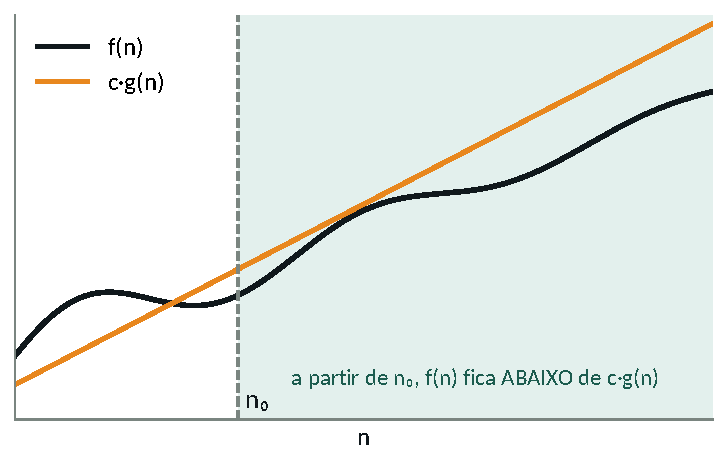
\includegraphics[width=0.72\textwidth]{figuras/f05_definicao_O.pdf}
  \caption{Antes de $n_0$, $f$ pode até passar do teto. Na região destacada, nunca mais.}
\end{figure}

\section{Exemplo guiado: \texorpdfstring{$3n + 4 = O(n)$}{3n + 4 = O(n)}}

Queremos mostrar que existe um par $(c, n_0)$ com $3n + 4 \le c \cdot n$ para todo $n \ge n_0$.

\begin{enumerate}
  \item \textbf{Escolha um $c$ um pouco maior que o coeficiente de $n$.} O coeficiente é 3;
        vamos tentar $c = 4$.
  \item \textbf{Resolva a desigualdade:} $3n + 4 \le 4n$ \ $\Longleftrightarrow$ \ $4 \le 4n - 3n$
        \ $\Longleftrightarrow$ \ $4 \le n$.
  \item \textbf{Leia o resultado:} a desigualdade vale para todo $n \ge 4$. Então $n_0 = 4$.
\end{enumerate}

Conferindo com números:

\begin{center}
\begin{tabularx}{0.9\textwidth}{L C C C C C C}
\cab \tcx{$n$} & \tc{1} & \tc{2} & \tc{3} & \tc{4} & \tc{5} & \tc{6} \\
$3n + 4$ & 7 & 10 & 13 & 16 & 19 & 22 \\
\rowcolor{edfundo} $4n$ & 4 & 8 & 12 & 16 & 20 & 24 \\
vale $3n + 4 \le 4n$? & não & não & não & \textbf{sim} & \textbf{sim} & \textbf{sim} \\
\end{tabularx}
\end{center}

\begin{figure}[!htb]
  \centering
  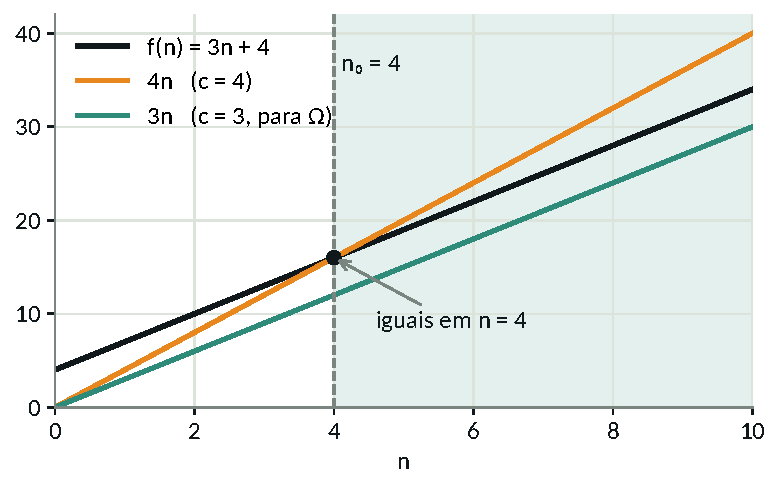
\includegraphics[width=0.7\textwidth]{figuras/f05_exemplo_3n4.pdf}
  \caption{$3n + 4$ fica abaixo de $4n$ a partir de $n_0 = 4$. (A reta $3n$ será usada no capítulo 6.)}\label{fig:exemplo3n4}
\end{figure}

Encontramos $c = 4$ e $n_0 = 4$; logo, $3n + 4 = O(n)$. Outros pares também servem: com $c = 7$,
por exemplo, a desigualdade $3n + 4 \le 7n$ vale desde $n_0 = 1$. A definição só pede que
\textbf{exista} um par.

\section{Uma técnica que sempre funciona para polinômios}

Para mostrar que $2n^2 + 3n + 1 = O(n^2)$: para $n \ge 1$, temos $n \le n^2$ e $1 \le n^2$.
Então podemos trocar cada termo pelo maior deles:
\[
2n^2 + 3n + 1 \;\le\; 2n^2 + 3n^2 + 1n^2 \;=\; 6n^2 \qquad \text{para todo } n \ge 1.
\]
Logo, $c = 6$ e $n_0 = 1$ funcionam. O truque: \textbf{some os coeficientes} e use o resultado
como $c$.

\section{Como mostrar que algo NÃO é \texorpdfstring{$O$}{O}}

Será que $n^2 = O(n)$? Se fosse, existiriam $c$ e $n_0$ com $n^2 \le c \cdot n$ para todo
$n \ge n_0$. Dividindo os dois lados por $n$ (que é positivo), isso vira $n \le c$. Mas $n$ cresce
sem parar e $c$ é fixo: basta tomar $n = c + 1$ (e maior que $n_0$) para a desigualdade falhar.
Nenhuma constante segura $n^2$ debaixo de $c \cdot n$. Portanto, $n^2$ \textbf{não} é $O(n)$.

\section{O é um teto — e pode ser folgado}

É verdade que $3n + 4 = O(n^2)$: um teto quadrático é alto o suficiente para uma função linear.
Mas essa informação é pobre, como dizer que \enquote{um carro custa menos que um bilhão de reais}.
Na prática, sempre buscamos o teto \textbf{mais justo} possível: $3n + 4 = O(n)$. Quando quisermos
dizer que o teto é exato, usaremos a notação $\Theta$ (capítulo 7).

\begin{atencao}
Três erros comuns:
\begin{itemize}
  \item Escrever $O(2n)$ ou $O(n^2 + n)$: as constantes e os termos menores devem ser removidos.
        Escreva $O(n)$ e $O(n^2)$.
  \item Achar que $O(n)$ quer dizer \enquote{exatamente $n$ passos}. Quer dizer \enquote{no máximo
        proporcional a $n$, para $n$ grande}.
  \item Achar que $O$ significa \enquote{pior caso}. $O$ é uma forma de comparar funções; o pior
        caso é uma situação dos dados. Voltaremos a isso nos capítulos 8 e 9.
\end{itemize}
\end{atencao}

\begin{exrapido}
Mostre que $2n + 10 = O(n)$, encontrando um par $c$ e $n_0$.
\end{exrapido}

\begin{exrapido}
(a) $7 = O(1)$? Encontre $c$ e $n_0$. (b) $n^2 + 100 = O(n^2)$? (c) $n^2 = O(n)$?
\end{exrapido}

\begin{respostas}
  \resp{5.1} Com $c = 3$: $2n + 10 \le 3n \Longleftrightarrow 10 \le n$. Então $c = 3$ e $n_0 = 10$.
  Outra resposta válida: com $c = 12$, $2n + 10 \le 12n$ vale desde $n_0 = 1$ (pela técnica de
  somar os coeficientes).
  \resp{5.2} (a) Sim: $7 \le 7 \cdot 1$ sempre, com $c = 7$ e $n_0 = 1$. Custo constante é $O(1)$.
  (b) Sim: $n^2 + 100 \le n^2 + 100n^2 = 101n^2$ para $n \ge 1$ ($c = 101$, $n_0 = 1$); ou
  $n^2 + 100 \le 2n^2$ para $n \ge 10$ ($c = 2$, $n_0 = 10$). (c) Não: veja a seção 5.5.
\end{respostas}
